\newpage

\section{Firewall}
There are different types of firewall, depending on what their job is. In this tutorial, you will be exposed to a firewall that is placed in a network. The firewall's job is to filter packets that are travelling through it and decide what should be done with the packets. More on that in the next section.

In this tutorial, you will be working with the \opnsense\ firewall. It is an open-source firewall solution that is developed by Deciso. A firewall can have other functions in a network than just filtering packets. Such jobs could be as a proxy server or a VPN server. The \opnsense\ firewall that you are going to work with within this tutorial, contains a lot of different features. For an overview of the features, go to \url{https://www.deciso.com/short-introduction-opnsense/}.

%\readblock{This is additional reading that will support you}

In this section, you will learn to:
\begin{itemize}
    \item Configure firewall rules.
    \item Logging of firewall rules.
    \item Best practice to achieve good throughput
    \item Create rules based on a time schedule.
    \item Geoblocking.
    \item And some tips and tricks regarding troubleshooting
\end{itemize}

\subsection{Firewall rules}
To go to the firewall rules, click on the \cmd{Firewall --> Rules} and then on the network interface you want the rules to apply (figure \ref{opnsense:firewall_rules}). In this case, rules can be applied to four different interfaces:
\begin{itemize}
    \item Floating - Rules that apply for all interfaces, and will be matched before any of the other interfaces, if the \cmd{Quick} checkbox is checked. Also, the only interface that allows \cmd{outbound} rules.
    \item LAN - Your internal pointing interface.
    \item Loopback - A interface that is used to communicate with the host (itself).
    \item WAN - Your external pointing interface.
\end{itemize}

\begin{figure}[h!]
    \centering
    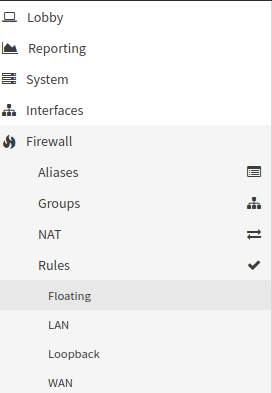
\includegraphics[width=0.3\textwidth]{Images/firewall/firewall_rules.PNG}
    \caption{\opnsense\ Firewall }
    \label{opnsense:firewall_rules}
\end{figure}

When \opnsense\ is processing rules, it is using the first rule it gets a match in. This is called the ''first match principle''. The rules are checked from the top of the list to the bottom. The basic rule for firewall ruleset is that the rule is acting one interface and filtering packets in the inbound direction. If you want to match in the outgoing direction or on multiple interfaces, floating rules need to be used.

\opnsense\ is a stateful firewall. This means that the firewall is remembering information about the outgoing packets and are automatically allowing the response from those packets back into the client that sent it.

% default deny any?

When creating rules in \opnsense\ three different types of actions can be done:
\begin{itemize}
    \item Pass - Allow the request.
    \item Block - Deny the request, but silently discards the request. Mostly used when you want the network to not know that the request has been denied, such as traffic from the internet.
    \item Reject - Deny the request, also discards the request, but lets the sender know it is discarded. Mostly used on requests from the internal network.
\end{itemize}

\quesblock{\begin{enumerate}
    \item[12.] Why do you think the action \cmd{Reject} is mostly used on so-called friendly networks?
\end{enumerate}}

\subsection{Creating first rule}
You are now set to create the first rule in the firewall. Follow the instructions below.

\setupblock{\begin{enumerate}
    \item First step is to start your Ubuntu Server that was created earlier in section \ref{ubuntu_server}.
    \item Make sure that the network in VMWare is set correct for the Ubuntu Server. Set to the virtual network that was created earlier.
    \item Use the Ubuntu Desktop and try to \cmd{PING} the Ubuntu Server. Continue if you can ping it.
    \item Ping any website that are online. If this works, continue.
    \item Goto \cmd{Firewall --> Rules --> LAN} and click on \cmd{Add}.
    \item Change the following settings:
    \begin{enumerate}
        \item \cmd{Action} to \cmd{Block}
        \item \cmd{TCP/IP Version} to \cmd{IPv4}
        \item \cmd{Direction} to \cmd{In}
        \item \cmd{Source} to \cmd{Single host or Network} and the IP below to the IP address that your Ubuntu Server has, and the correct CIDR (Classless Inter-Domain Routing).
        \item Click the box next to \cmd{Log} to log the rule.
        \item In the \cmd{Descripion} box, write what this rule is. For example, ''Block <IP> from internet access.''
        \item Click \cmd{Save} at the bottom and apply the rule when asked.
    \end{enumerate}
\end{enumerate}}

\quesblock{\begin{enumerate}
    \item[13.] Try now to \cmd{PING} the same website as you did in bullet point 4. What is happening?
    \item[14.] How can you disable the rule that was created?
    \item[15.] Are you able to ping any website from the Ubuntu Server when the rule is disabled? 
\end{enumerate}}

\tipbox{To stop the \cmd{PING} command, use the keyboard keys \cmd{CTRL-C} to stop it, or use the option \cmd{-c 3} to ping the server 3 times.}

Play around with the different settings and try to understand how the rules are created.

% more examples?

\subsubsection{Logging}
Each of the rules can be logged. To log a rule, click on the \cmd{Log packets that are handled by this rule} to add the rule to the logs. The best practice is to use logging only on critical rules, such as anti-spoofing or critical segments of the network, like a DMZ. Turn logging on and off after what the user needs. For example, logging is great for troubleshooting.

\warnblock{\textbf{Be aware that the logs can fill up fast when this is applied and the rule is handling a lot of traffic. }}

There are three different ways to see the information from the logs. The first one is \cmd{Live view}. This is showing the user a live view of the log entries. When a new entry is made, it will appear at the top, and the one at the bottom will go to the next page in the log. This happens in real-time. The second view is the \cmd{Overview}. This is a more graphical presentation of what is going on in the logs. The last view is the \cmd{Plain view}. This is more like a command line like view. 

An example can be seen in figure \ref{opnsense:firewall_log}. First is the Data, then the process that wrote the entry. Under the \cmd{Line} column, there is a lot of information. Some of them are which interface is used (em0), the reason for the log entry (match), what the rule did (block), the direction of communication (in) and the protocol and IP source and destination.

\begin{figure}[h!]
    \centering
    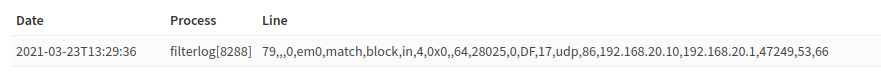
\includegraphics[width=0.9\textwidth]{Images/firewall/log.PNG}
    \caption{\opnsense\ Firewall log; Plain view}
    \label{opnsense:firewall_log}
\end{figure}

\quesblock{\begin{enumerate}
    \item[16.] Do you see any evidence in the log when the first rule that was created earlier is active? 
\end{enumerate}}

\subsection{Second firewall rule}
For this second rule, the goal is to block all LAN traffic and allow connection to the Ubuntu Server using the 8080 port. First, we are disabling the two default rules that allow all LAN traffic.

\setupblock{\begin{enumerate}
    \item Go to \cmd{Firewall --> Rules --> LAN}.
    \item Click on the green right arrow for both default allow LAN to any rules (IPv4 and IPv6). When this is done, the rules should look like figure \ref{opnsense:default_allow_disable}, the arrows greyed out.
    \item Click on \cmd{Add} to add a rule.
    \item Change the following settings:
    \begin{enumerate}
        \item \cmd{Action} to \cmd{Pass}
        \item \cmd{TCP/IP Version} to \cmd{IPv4}
        \item \cmd{Direction} to \cmd{In}
        \item \cmd{Source} to \cmd{Single host or Network} and the IP below to the IP address that your Ubuntu Server has, and the correct CIDR (Classless Inter-Domain Routing).
        \item Click the box next to \cmd{Log} to log the rule.
        \item In the \cmd{Descripion} box, write what this rule is. For example, ''Allow \textless IP\textgreater to use port 8080.''
        \item \cmd{Source port range} to \cmd{other} and from port \cmd{8080} to port \cmd{8080}.
        \item \cmd{Destination} to \cmd{Any}
        \item \cmd{Destination port range} to \cmd{any}.
        \item Make a checkmark in the checkbox beside \cmd{Log}.
        \item Click \cmd{Save} at the bottom and apply the rule when asked.
    \end{enumerate}
\end{enumerate}}

\begin{figure}[h!]
    \centering
    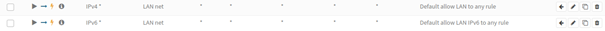
\includegraphics[width=1\textwidth]{Images/firewall/default_allow_rules.png}
    \caption{Default allow LAN rules disabled}
    \label{opnsense:default_allow_disable}
\end{figure}

\quesblock{\begin{enumerate}
    \item[17.] How can you test if this is working?
    \item[18.] Play around and try to create other rules. 
\end{enumerate}}

\tipbox{Remember to enable the two default allow rules before continuing with the tutorial}

\warnblock{If you have problems when testing the rule that was created, try to restart the service used for testing purposes on the Ubuntu Server after each time the rule is enabled/disabled.}

\subsection{Thrughput and best practice}
Some basic rules to keep the ruleset as close to best practice as possible (\cite{Stubbig2019}) regarding throughput.

\begin{itemize}
    \item Keep it simple - Do not make it complicated. Complicated rules are only working until the next time you change something.
    \item Documentation - Document rules. Each rules has an \cmd{description} field.
    \item Aliases - Merge everything that has the same rules into groups.
    \item Use source network - If the rule allows traffic, choose the source network. If the rule is denying traffic, choose any as the source.
    \item IPv4 and IPv6 - It is possible to use one rule for both. Remember to add both the IPv4 and IPv6 address to aliases if it is used.
    \item Use inbound rules - It is possible to use inbound and outbound rules, but the best practice is to use inbound rules. An outbound rule can be created using the floating rule.
    \item Audit - Audit regularly. Goto \cmd{Firewall --> Diagnostics --> pfInfo} to see statistics about each rule. Assess if rules that are not used, should be removed.
\end{itemize}

\subsubsection{Rulesets best prasctice}
To make the rulesets as effective as possible, use this as a guideline for how to implement a strategy of which rules should be first in the hierarchy (which rule is matched first):
\begin{enumerate}
    \item Anti-spoofing rules - block bogus addresses. See section \ref{anti_spoofing}.
    \item Special rules - Rules that are specific for IP's, and ports.
    \item General rules - Rules that are for networks and/or ports.
    \item Cleanup rules - A rule to clean up events that should not be in a log.
    \item Final-deny-any-log - Block everything that is left and log anything that hit this rule.
\end{enumerate}

\subsection{Time-based rules}
In \cmd{Firewall --> Settings --> Schedule} there can be configured schedules that are based on time and day. Those schedules can be added to any firewall rule. This can be smart, for example, if a company is blocking specific pages during periods of the day to minimize the load on the outgoing network.

\quesblock{\begin{enumerate}
    \item[19.] Where in the rule editor page can you add the time-based rule?
    \item[20.] Try to create a schedule and add it to a rule that blocks access to \cmd{www.nrk.no} inside the normal working hours (08.00 - 16.00). % Make an example for the answers.
\end{enumerate}}

\subsection{Anti-spoofing} \label{anti_spoofing}
As standard, the \opnsense\ firewall can detect a spoofed IP from network adapters. It creates a hidden rule that detects and blocks incoming traffic, where the source IP belongs to some of the other adapters.

If the firewall has multiple networks to an adapter, a rule needs to be created to block spoofed IP's. First, create an alias with all of the networks that are behind the adapter. Then create a rule that blocks all traffic from the alias that was created, but inverted. This will deny all incoming traffic on that alias that does not originate from the alias.

% Test this!! the book has a bad description of this.

\subsection{Geoblocking}
The geo blocking feature in \opnsense\ is using the MaxMind GeoIP database. So the first step is to create an account for it:
\setupblock{\begin{enumerate}
    \item Go to \url{https://www.maxmind.com/en/geolite2/signup} and sign up.
    \item Log in on your account and find the \cmd{My License Key} link and generate the license key.
    \item To create a link, replace \cmd{My\_License\_key} with the license key you generated in the previous step in \url{https://download.maxmind.com/app/geoip_download?edition_id=GeoLite2-Country-CSV&license_key=My_License_key&suffix=zip}.
    \item Goto \cmd{Firewall --> Aliases} and choose the \cmd{GeoIP Settings} tab. 
    \item In the \url{Url} insert the link you created in step 3, and click \cmd{Apply} to finish.
\end{enumerate}}

Now the connection to MaxMind GeoIP database is finished. The next step is to greate an alias that is using it.
\setupblock{\begin{enumerate}
    \item Go to \cmd{Firewall --> Aliases}. Click the \cmd{+} sign to add a new alias.
    \item Set the \cmd{Name} to the something that describes what it does. For example, \cmd{block <countryname>}
    \item Set \cmd{Type} to \cmd{GeoIP}
    \item Choose the country you want to block.
    \item Set the \cmd{Description} to something that describes what it do. In this case to the same as the \cmd{Name} could be great.
    \item Click \cmd{Save} to exit and save the alias.
\end{enumerate}}

The alias is made and the last step is to create a rule in the firewall that is blocking that alias.

\quesblock{\begin{enumerate}
    \item[21.] Can you create a firewall rule that uses the alias you created to block one country?
    \item[22.] How can you test if the previous create rule is working?
\end{enumerate}}

\tipbox{Remember that the order of the rules matter. If you, for example, want to access one website from the country that you are blocking, the allow rule needs to be before the block rule.}

\subsection{Throubleshooting rules}
If a rule is not behaving as expected, the steps below can help you to figure out what is happening:
\begin{enumerate}
    \item Check the logic of your rules. Check if it is using the correct interface, ports, IP, protocols, and so on.
    \item Are the rules in the correct order? Rules are processed from the top to the bottom.
    \item Floating rules are processed before other firewall rules. Check if some of them are hindering your new rule.
    \item Does NAT (Native Translation Protocol) modify packets?
    \item Is the routing done correctly?
    \item Check the logs to check what is going on.
\end{enumerate}

\quesblock{\begin{enumerate}
    \item[23.] Is it possible to do a packet capture with \opnsense?
\end{enumerate}}
